\subsection{生成剖视图}
\begin{procedure}
\item 打开“调压阀阀体立体图.dwg”文件,并另存为“调压阀阀体布局图.dwg”。
\item 创建布局。
\item 创建基础俯视图,结果如图\ref{fig:fativiewbase1}所示。
\begin{figure}[htbp]
\centering
\begin{floatrow}[2]
\ffigbox{\caption{生成俯视图}\label{fig:fativiewbase1}}{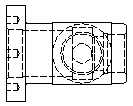
\includegraphics[scale=1]{fativiewbase1.png}}
\ffigbox{\caption{生成全剖主视图}\label{fig:fativiewbase2}}{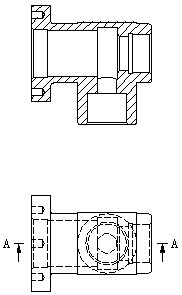
\includegraphics[scale=1]{fativiewbase2.png}}
\end{floatrow}
\end{figure}
\begin{lstlisting}
|命令: VIEWBASE|
|指定模型源 [模型空间(M)/文件(F)] $<$模型空间$>$:|
|选择对象或 [整个模型(E)] $<$整个模型$>$: 找到 1 个|
|选择对象或 [整个模型(E)] $<$整个模型$>$:|
|输入要置为当前的新的或现有布局名称或 [?]$<$布局3$>$:|
|正在重生成布局。|
|正在重生成布局。|
|类型 = 基础和投影  隐藏线 = 可见线和隐藏线  比例 = 1:2|
|指定基础视图的位置或 [类型(T)/选择(E)/方向(O)/隐藏线(H)/|
|比例(S)/可见性(V)] $<$类型$>$:o|
|选择方向 [当前(C)/俯视(T)/仰视(B)/左视(L)/右视(R)/前视(F)/|
|后视(BA)/西南等轴测(SW)/东南等轴测(SE)/东北等轴测(NE)/|
|西北等轴测(NW)] $<$前视$>$: t|
|选择选项 [选择(E)/方向(O)/隐藏线(H)/比例(S)/可见性(V)/|
|移动(M)/退出(X)] $<$退出$>$:|
|指定投影视图的位置或 $<$退出$>$:|
\end{lstlisting}
\item 创建全剖主视图,结果如图\ref{fig:fativiewbase2}所示。
\begin{lstlisting}
|命令: VIEWSECTION|
|选择父视图:找到 1 个|
|隐藏线 = 可见线 比例 = 1:2 (来自父视图)|
|指定起点或 [类型(T)/隐藏线(H)/比例(S)/可见性(V)/注释(A)/|
|图案填充(C)] $<$类型$>$:|
|指定下一个点或 [放弃(U)]:|
|指定下一个点或 [放弃(U)/完成(D)] $<$完成$>$:|
|指定截面视图的位置或:|
|选择选项 [隐藏线(H)/比例(S)/可见性(V)/投影(P)/深度(D)/注释(A)/|
|图案填充(C)/移动(M)/退出(X)] $<$退出$>$: X|
\end{lstlisting}

\item 以俯视图为父视图创建半剖视图,结果如图\ref{fig:fativiewbase3}所示。
\begin{figure}[htbp]
\centering
\begin{floatrow}[2]
\ffigbox{\caption{生成半剖视图}\label{fig:fativiewbase3}}{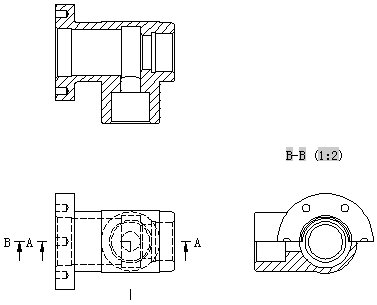
\includegraphics[scale=0.6]{fativiewbase3.png}}
\ffigbox{\caption{旋转半剖视图}\label{fig:fativiewbase4}}{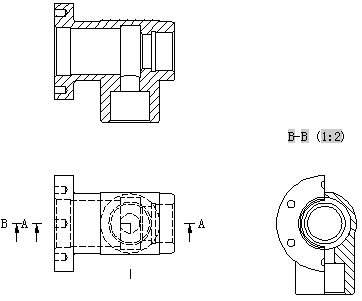
\includegraphics[scale=0.6]{fativiewbase4.png}}
\end{floatrow}
\end{figure}
\begin{lstlisting}
|命令: VIEWSECTION|
|选择父视图:找到 1 个|
|隐藏线 = 可见线 比例 = 1:2 (来自父视图)|
|指定起点或 [类型(T)/隐藏线(H)/比例(S)/可见性(V)/注释(A)/|
|图案填充(C)] $<$类型$>$: t|
|选择类型 [全剖(F)/半剖(H)/阶梯剖(OF)/旋转剖(A)/对象(OB)/|
|退出(X)] $<$退出$>$: h|
|指定起点:|
|指定下一个点或 [放弃(U)]:|
|指定端点或 [放弃(U)]:|
|指定截面视图的位置或:|
|选择选项 [隐藏线(H)/比例(S)/可见性(V)/投影(P)/深度(D)/注释(A)/|
|图案填充(C)/移动(M)/退出(X)] $<$退出$>$: X|
\end{lstlisting}
\item 旋转半剖视图。

由于生成的半剖视图的位置不正确,需要按照国家标准规定的三视图位置将半剖视图调整到正确的位置。因此先将其逆时针旋转90度,然后再移动到正确的视图位置。进行视图旋转需要用到旋转命令,其启动方法有:
\begin{itemize}
\item 键盘输入ROTATE\index{rotate,旋转}或RO。
\item 【修改】$\rightarrow$【旋转】。
\item 【修改】$\triangleright$【旋转】图标
\includegraphics[scale=0.6]{rotate.png}。
\end{itemize}

启动旋转命令后选择半剖视图为旋转对象。
\begin{lstlisting}
|命令: ROTATE|
|UCS 当前的正角方向:  ANGDIR=逆时针  ANGBASE=0|
|选择对象: 找到 1 个|
|选择对象:|
\end{lstlisting}
选择半剖视图中圆的圆心为基点,亦可选择其它点。
\begin{lstlisting}
|指定基点:|
\end{lstlisting}
指定旋转角度为90度。通常情况下,若角度为负值,则为旋转方向为时针,正值则为逆时针。其旋转结果如图\ref{fig:fativiewbase4}所示。
\begin{lstlisting}
|指定旋转角度,或 [复制(C)/参照(R)] $<$0$>$:  90|
\end{lstlisting}
\item 移动半剖视图到左视图位置。

为确保将半剖视图移动到符合三视图投影规律的标准位置,需要先绘制一根定位辅助线,结果如图\ref{fig:fativiewbase5} 所示。
\begin{lstlisting}
|命令: line|
|指定第一个点: mid 于|
|指定下一点或 [放弃(U)]:  $<$正交 开$>$|
|指定下一点或 [放弃(U)]:|
\end{lstlisting}
\begin{figure}[htbp]
\centering
\begin{floatrow}[2]
\ffigbox{\caption{绘制定位辅助线}\label{fig:fativiewbase5}}{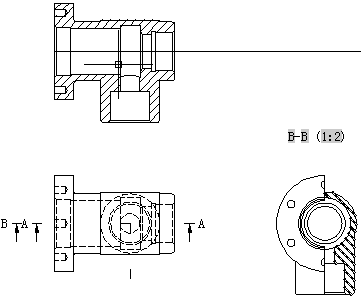
\includegraphics[scale=0.6]{fativiewbase5.png}}
\ffigbox{\caption{移动半剖视图}\label{fig:fativiewbase6}}{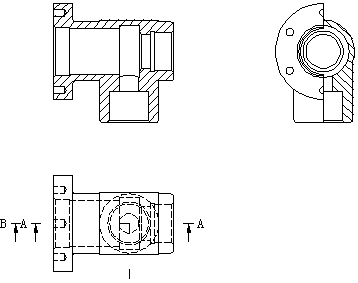
\includegraphics[scale=0.6]{fativiewbase6.png}}
\end{floatrow}
\end{figure}
选择半剖视图中的圆心为移动基点,将其移到定位辅助线上。
\begin{lstlisting}
|命令: MOVE|
|选择对象: 找到 1 个|
|选择对象|:
|指定基点或 [位移(D)] $<$位移$>$:|
|指定第二个点或 $<$使用第一个点作为位移$>$: near 到|
\end{lstlisting}
删除定位辅助线。删除命令的启动方法有:
\begin{itemize}
\item 键盘输入ERASE\index{erase,删除}或E。
\item 【修改】$\rightarrow$【删除】。
\item 【修改】$\triangleright$【删除】图标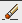
\includegraphics[scale=0.6]{erase.png}。
\end{itemize}
\begin{lstlisting}
|命令:ERASE|
|选择对象: 找到 1 个|
|选择对象:|
\end{lstlisting}
\end{procedure}
通过上述步骤,即可完成半剖左视图的生成,结果如图\ref{fig:fativiewbase6}所示。
\endinput